% mycsrf 'for beeing included' snippet template
%
% (c) Karsten Reincke, Frankfurt a.M. 2012, ff.
%
% This text is licensed under the Creative Commons Attribution 3.0 Germany
% License (http://creativecommons.org/licenses/by/3.0/de/): Feel free to share
% (to copy, distribute and transmit) or to remix (to adapt) it, if you respect
% how you must attribute the work in the manner specified by the author(s):
% \newline
% In an internet based reuse please link the reused parts to mycsrf.fodina.de
% and mention the original author Karsten Reincke in a suitable manner. In a
% paper-like reuse please insert a short hint to mycsrf.fodina.de and to the
% original author, Karsten Reincke, into your preface. For normal quotations
% please use the scientific standard to cite
%


%% use all entries of the bibliography

\subsection{Denemo ($\bigstar\bigstar\bigstar$)}

\parpic(1cm,1cm)[r][t]{
\includegraphics[width=1cm]{logos/denemo-300dpi.png}}
\label{Denemo}\acc{LilyPond} bezeichnet \acc{Denemo} als \enquote{graphischen
Editor} und bietet ihn -- nach \acc{Frescobaldi} -- an zweiter Stelle seiner
Liste von Programmen an, die das Editieren erleichtern sollen. Hervorgehoben
wird hier, dass \acc{Denemo} -- neben der graphischen Manipulation des
Notenbildes -- auch das Editieren des \acc{LilyPond}-Quelltextes erlaube und
zugleich das per \acc{LilyPond} erzeugte PDF anzeige.\footcite[vgl.][\nopage
wp.]{LilyPond2018g} Damit wäre \acc{Denemo} ein graphischer und ein
semi-graphischer Editor.

\acc{Denemo} selbst sagt von sich, dass die Musik via Tastatur, MIDI-Controller
oder Mikrophon eingegeben werden könne und dass das eine Methode sei,
\enquote{[\ldots] to enter music in a musical, rather than mechanical,
manner}.\footcite[vgl.][\nopage wp.]{Denemo2019b} Tatsächlich wird die Musik hier
visuell und per Tastatur editiert: zuerst markiert man mit der Maus und dem
Cursor eine Stelle, erhält damit einen Eingabemodus und sagt dann per Tastatur,
was an dieser Stelle erscheinen resp. verändert werden solle.\footcite[vgl.][1,
5, u. 47ff]{Shann2015b} Dies zu verstehen und den Cursor entsprechend zu nutzen,
ist die eine Hürde, die man nehmen muss, wenn man \acc{Denemo} produktiv
einsetzen will.

In der Regel wird dieses Programm von gängigen Distributionen als fertig
intergiertes Paket mitgeliefert.\footcite[vgl. z.B.][\nopage
wp.]{UbuntuDenemo2014a} Seine Homepage stellt jedoch auch eigenständige
Versionen für GNU/Linux und Windows bereit.\footcite[vgl.][\nopage
wp.]{Denemo2019d} Und als GPL lizenzierte freie Software werden auch seine
Quellen in einem Repository gehostet und öffentlich
weiterentwickelt.\footnote{\cite[vgl.][\nopage wp.]{GithubDenemo2019a}.
Das Repository enthält unter dem namen 'COPYING' die GPL-3.0-Lizenz, die
\acc{Denemo} damit als echte freie Software ausweist. Darüber hinaus ist
\acc{Denemo} sogar Teil des GNU-Projektes ( $\rightarrow$
\\href{https://www.gnu.org/software/} {https://www.gnu.org/software/})}

Ein Handbuch erläutert die Nutzung von \acc{Denemo}. Es liegt in einer
Online-Version\footcite[vgl.][\nopage wp.]{Shann2015a} und in einer
PDF-Version vor.\footcite[vgl.][2ff]{Shann2015b} Beide sind allerdings schwer zu
lesen und nicht unbedingt leicht zu verstehen -- ersteres aber wenigstens leichter
zu durchsuchen. Daneben bietet \acc{Denemo} noch eine FAQ-Seite
an.\footcite[vgl.][\nopage wp.]{Denemo2019c} Ohne sich diese Anleitungen
wenigstens in Grundzügen anzueignen, wird man keine Freude an dem Programm
haben: sie zu lesen, -- und das ist die zweite Hürde -- ist allerdings selbst
kaum ein Genuss.

Die dritte Hürde ist die Integration des Programms in bestehende Desktopsysteme:
\acc{Denemo} erlaubt, Teile seines Menues 'abzureißen' und als Paletten in Form
eigener Fenster zu behandeln. Unglücklicherweise geht damit oft der Fensterfokus
verloren. Das \acc{Denemo}-Menue überlagert dann noch das Fenster anderer
Programme, wenn diese längst den Fokus erhalten haben. Ein flüssiges
gleichzeitiges Arbeiten mit z.B. einem \LaTeX-Editor und mit \acc{Denemo} ist
-- enttäuschenderweise -- so nicht wirklich möglich.

\acc{Denemo} verwendet \acc{LilyPond als Backend}.\footcite[vgl.][\nopage
wp.]{Denemo2019b} Trotzdem speichert es seine Dateien in erster Linie in einem
eigenen XML-Format. Die entsprechenden Dateien tragen die Extension
\texttt{.denemo}.\footcite[vgl. dazu][\nopage wp.]{WpedDenemo2018a} Über sein
Menue bietet \acc{Denemo} -- wie es dort selbst anzeigt -- einen 'begrenzten'
Import von \acc{LilyPond}- und \acc{MIDI}-Dateien und einen uneingeschränkten
Import von \acc{MusicXML}-Dateien. Zum Export stehen -- wie kaum anders zu
erwarten -- alle Formate bereit, die mit \acc{LilyPond} generiert werden können,
also die \acc{LilyPond}-Dateien selbst und die entsprechende Graphik- und
\acc{MIDI}-Versionen. Außerdem bietet \acc{Denemo} den Export als Audio-Datei an.

Tatsächlich ist es uns überhaupt nicht gelungen, die \acc{LilyPond}-Version
unser Referenzkadenz II nach  \acc{Denemo} zu importieren, die \acc{Frescobaldi}
problemlos hat nutzen können. Der Import der von \acc{Frescobaldi} /
\acc{LilyPond} generierten \acc{MIDI}-Datei war formal möglich, stimmte aber
inhaltlich nicht. Erst der Import einer \acc{MusicXML}-Datei ohne textuelle
Analysesymbole gelang erwartungsgemäß.

\begin{center}
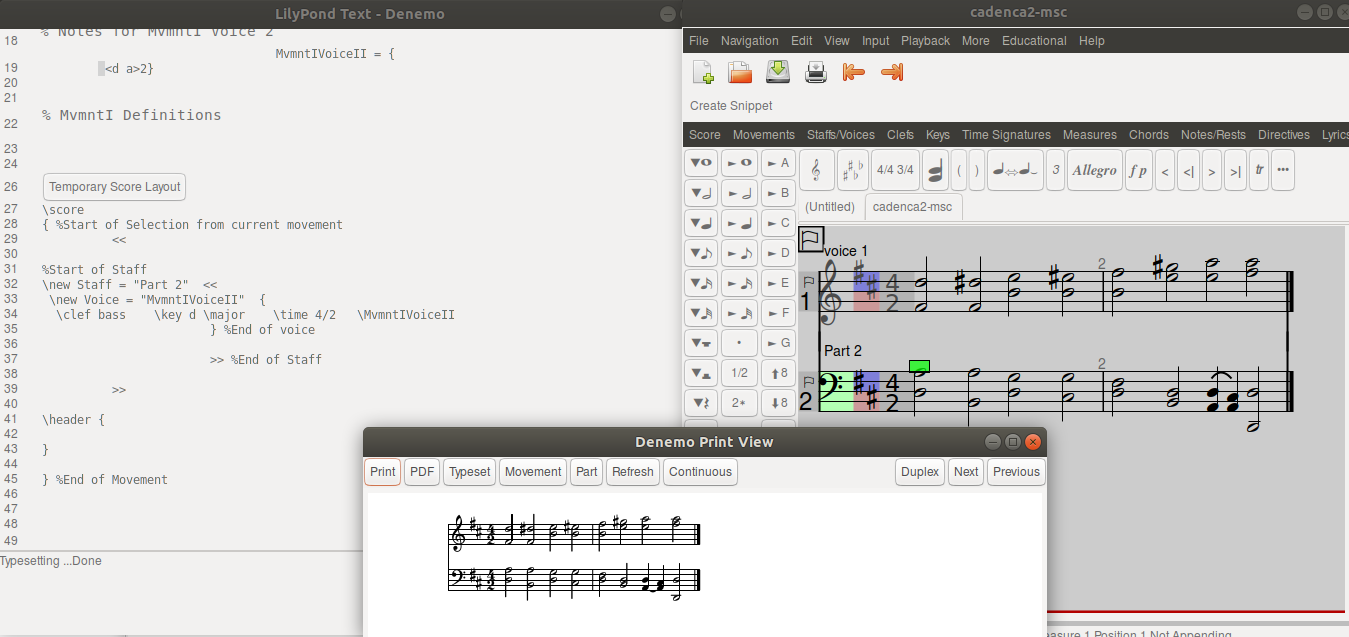
\includegraphics[width=0.9\textwidth]{frontends/denemo/denemo-cadenca2-300dpi.png}
\end{center}

Leider war es danach nicht möglich, die Symbole der Harmonyanalyse in den
Notentext zu integrieren. Dass wir dazu unsere kleine Zusatzbibliothek über den
\acc{LilyPond}-Editor hätten nutzen können, hatten wir nach den ersten
Erfahrungen realistischerweise schon nicht mehr angenommen. Dass dieser Editor in
seinem spartanischen Design die \acc{LilyPond}-Kodierung nur rudimentär
unterstützt, hätte dabei kaum geholfen. Dass aber \acc{Denemo} mit seinen
eigenen Mitteln auch nicht dazu zu überreden war, eine vereinfachte Version der
Harmonieanalyse in Form von 'Liedtext' zu erfassen, hatten wir nicht erwartet.

Insgesamt hat \acc{Denemo} eine lange Geschichte. Das ist im Rahmen freier
Software an sich ein Verdienst. Oft werden dann allerdings auch
programmiertechnische Altlasten mitgeschleppt, die ein modernes Design
und eine Integration in moderne Systeme behindern. Darunter scheint \acc{Denemo}
zu leiden.

Für Musikwissenschaftler, die bereits mit dem Programm vertraut sind, kann es
als Noteneditor dienen. Die Analysesymbole wird er aber nachgelagert einfügen
müssen. Für Neueinsteiger scheinen Lern- und Arbeitsaufwand auf der einen Seiten
und die Qualität der Ergebnisse -- verglichen mit anderen freien Programmen --
nicht (mehr) in einem angemessenen Verhältnis zu stehen. Wenn \acc{Denemo} sich
wirklich einmal zum \enquote{Ziel} gesetzt hat, \enquote{[\ldots] effektiv und
in hoher Geschwindigkeit Notation für den LilyPond Music Engraver zu erstellen}
\footcite[vgl.][\nopage wp.]{WpedDenemo2018a}, dann muss man man ihm heute
attestieren, dass es seinen Nutzern dabei hohe Hürden zu überwinden auferlegt
hat. Wir sind daran gescheitert und geben \acc{Denemo} deshalb drei Sterne:
mehr als dem Uraltprogramm \acc{NtEd} und weniger als \acc{Elysium} oder gar 
\acc{Frescobaldi} und \acc{MuseScore}.
% this is only inserted to eject fault messages in texlipse
%\bibliography{../bib/literature}
